\documentclass[12pt]{article}
\usepackage{graphicx}
\usepackage{subcaption}
\setlength{\parindent}{0pt}
\setlength{\parskip}{10pt} % block paragraphs
\usepackage{bm}
\begin{document}

\title*{\centerline{\huge{CAP 5619 \-- Deep and Reinforcement Learning}}}
\author*{\centerline{Project1 Hua Huang}}%unnumbered centered head

\section{Task I-Neural Network Design}
In these 3 networks, reLU are adopted except for the 1st layer. Since
reLU is generally recognised as the best choice for most of the
application scenarios of Neural Network, it does not saturate when it
is fired, and derivative is always 1 if fired. This choice of
activation functions can guarantee in the backpropogation, the
gradients can be propogated to the deeper layer and hence the network
can be trained efficiently.\\
(1) Fully connected Neural Network. There are 4 layers(exclude the
input layer). The 1st layer has 256 units, activation function is
tanh. The 2nd and 3rd layer has 256 units, and the activation function
is reLU, the last layer is a softmax layer, which output the scores
for each of the 10 classes. In total, there are 199946 parameters.\\
(2) Locally connected with no weights shared in the first three
layers, where each neural/input is connected to the neurons in a local
neighbor in the next layer. There are 4 layers, the 1st layer has 8
filters, each filter has a size of $[3,3]$, and the activation function is
sigmoid. The 2nd and 3rd layer also has 8 filters, each of size $[3,3]$, and 
the activation function is reLU. The last layer is a softmax layer,
which output the scores for each of the 10 classes. In total, 
There are 166186 parameters.\\
(3) CNN. There are 4 layers, the 1st layer has 8
filters, each filter has a size of $[3,3]$, and the activation function is
sigmoid. The 2nd and 3rd layer also has 8 filters, each of size $[3,3]$, and 
the activation function is reLU. The last layer is a softmax layer,
which output the scores for each of the 10 classes. In total, 
There are 9258 parameters.\\

\section{Techniques for Optimization}
\subsection{parameter initialization strategies}
(1) Fully connected NN (MLP): The frist 3 layers are initialized as
\textit{Identity(gains=3.)}, the last layer is initialized as
\textit{TruncatedNormal(mean=0.0, stddev=0.05)}, the biases are
initialized as \textit{Constant(value=0.5)}.\\
To test the parameter choice, 3 \textit{gains} of $[0.1, 3, 10]$ are
tested, the performance is given in Fig.1, we can see \textit{gains=3}
is most appropriate among these 3, \textit{gains=0.1} will lead to
very slow learning, and \textit{gains=10} is too fast, it learns
within 10 epochs, after that, it never learns anymore.\\
\begin{figure}[h]
    \centering
    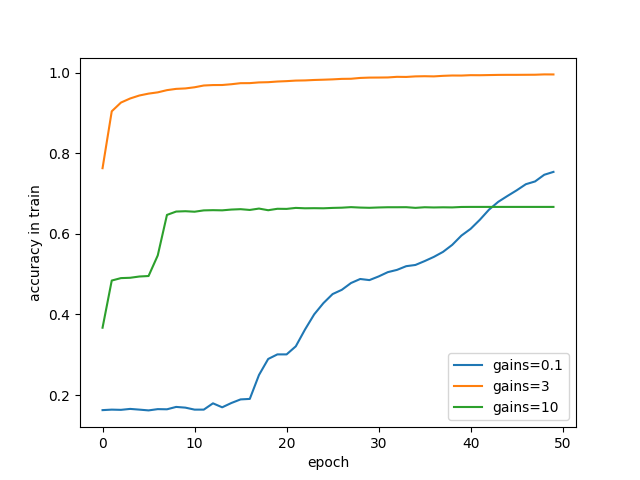
\includegraphics [scale=0.5]{mlp_initialization_accuracy.png}
    \caption {initialization in MLP}
\end{figure}

(2) Locally connected NN: All the 4 layers are initialized as
\textit{TruncatedNormal(mean=0.0, stddev=0.1)}, the biases are
initialized as \textit{Constant(value=0.5)}.\\
To test the parameter choice, 3 \textit{stddev} of $[0.15, 0.1, 0.05]$ are
tested, the performance is given in Fig.2, we can see \textit{stddev=0.1}
is most appropriate among these 3, \textit{stddev=0.05} will lead to
very slow learning, and \textit{stddev=0.15} is too fast, it learns
within 1 spoch, after that, it never learns anymore.
\begin{figure}[h]
    \centering
    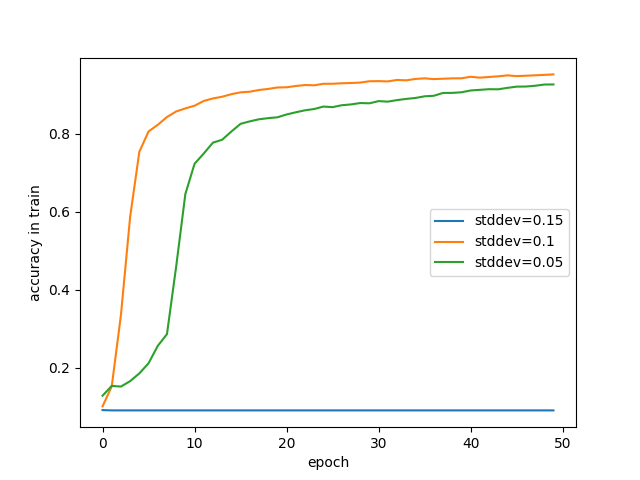
\includegraphics [scale=0.5]{local_initialization_accuracy.png}
    \caption {initialization in locally connected layer}
\end{figure}

(3) CNN: All the 4 layers are initialized as
\textit{TruncatedNormal(mean=0.0, stddev=0.1)}, the biases are
initialized as \textit{Constant(value=0.5)}.\\
To test the parameter choice, 3 \textit{stddev} of $[1.0, 0.5, 0.02]$ are
tested, the performance is given in Fig.3, we can see \textit{stddev=0.5}
is most appropriate among these 3, \textit{stddev=0.02} will lead to
very slow learning, and \textit{stddev=1.0} is too fast, it learns
within 1 spoch, after that, it never learns anymore.
\begin{figure}[h]
    \centering
    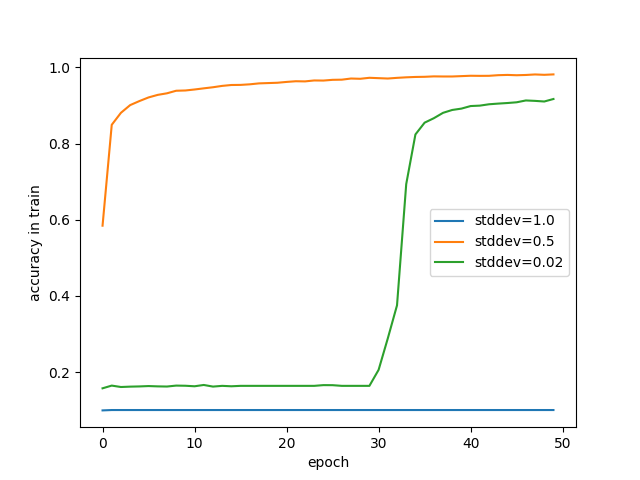
\includegraphics [scale=0.5]{cnn_initialization_accuracy.png}
    \caption {initialization in CNN}
\end{figure}

\subsection{learning rate}
(1) Fully connected NN (MLP): To test the parameter choice, 3 \textit{lr} of 
$[0.25, 0.01, 0.00001]$ are tested, the performance is given in Fig.4, 
we can see \textit{lr=0.01} is most appropriate among these 3, 
\textit{lr=0.00001} will lead to very slow learning, and \textit{lr=0.25} is 
too fast, it learns within 10 epochs, after that, it never learns anymore.\\
\begin{figure}[h]
    \centering
    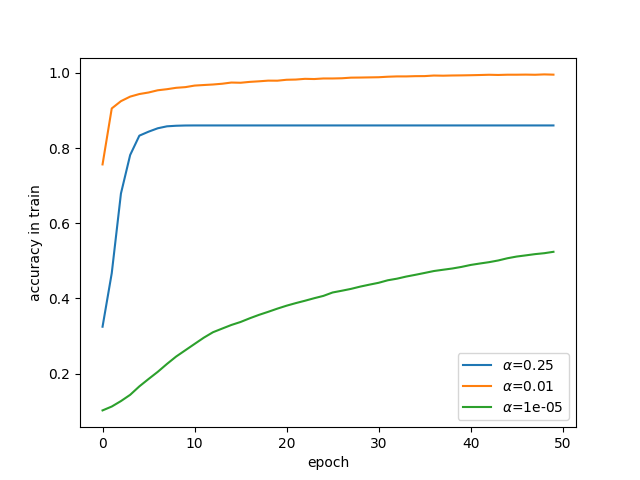
\includegraphics [scale=0.5]{mlp_stepsize_accuracy.png}
    \caption {step size in MLP}
\end{figure}

(2) Locally connected NN: To test the parameter choice, 3 \textit{lr} of
$[0.5, 0.1, 0.01]$ are tested, the performance is given in Fig.5, we can see
\textit{lr=0.1} is most appropriate among these 3, \textit{lr=0.01} will lead to
very slow learning, and \textit{lr=0.5} is too fast, it learns
within 1 spoch, after that, it never learns anymore.
\begin{figure}[h]
    \centering
    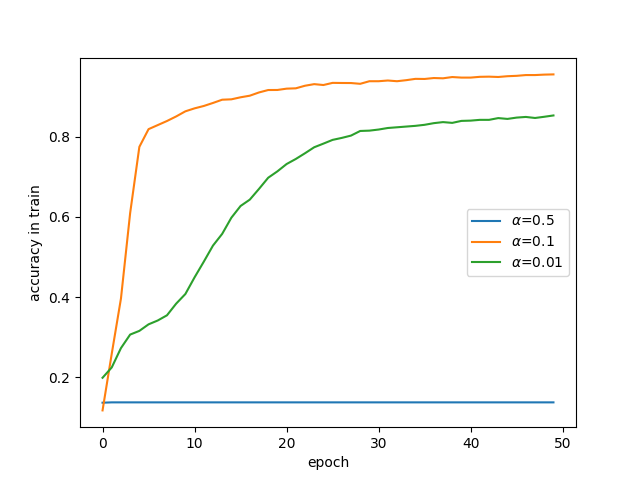
\includegraphics [scale=0.5]{local_stepsize_accuracy.png}
    \caption {stepsize in locally connected layer}
\end{figure}

(3) CNN: To test the parameter choice, 3 \textit{lr} of $[0.1, 0.01, 0.00001]$ are
tested, the performance is given in Fig.6, we can see \textit{lr=0.01}
is most appropriate among these 3, \textit{lr=0.00001} will lead to
very slow learning, and \textit{lr=0.1} is too fast, it learns
within 1 spoch, after that, it never learns anymore.
\begin{figure}[h]
    \centering
    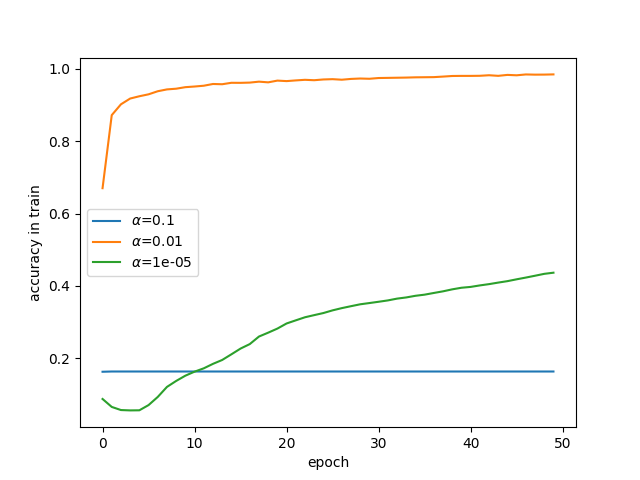
\includegraphics [scale=0.5]{cnn_stepsize_accuracy.png}
    \caption {step size in CNN}
\end{figure}

\subsection{Batch size effects}
If we do not consider the computational benefits, batch size is the
smaller the better. Although large batch size will lead to a more
accurate computation of the gradient, generally large batch size will
lead to bad performance. The behind reason is guessed to be that since
Neural Network is non\--convex optimization, the noise(or we can say
the inaccuracy) introduced by small\--size batch learning can help the
trainning escape the local optimum and hence obtain better
performance.\\
(1) Fully connected NN (MLP): To test the parameter choice, 2 \textit{batch size} of 
$[256, 8192]$ are tested, the performance is given in Fig.7, 
we can see \textit{batch size=256} is more appropriate, and 
\textit{batch size=8192} will lead to slow learning and bad final performance.\\
\begin{figure}[h]
    \centering
    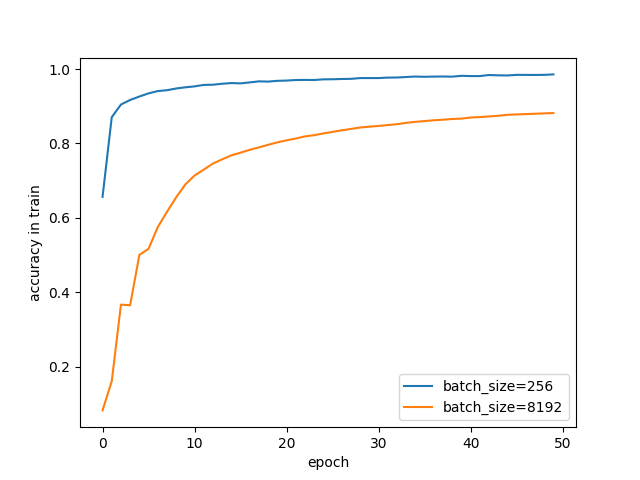
\includegraphics [scale=0.5]{mlp_batch_size_accuracy.png}
    \caption {batch size in MLP}
\end{figure}
\newpage

(2) Locally connected NN: To test the parameter choice, 2 \textit{batch size} of
$[128, 2048]$ are tested, the performance is given in Fig.8, we can see
\textit{batch size=128} is more appropriate, and 
\textit{batch size=2048} will lead to slow learning and bad final performance.\\
\begin{figure}[h]
    \centering
    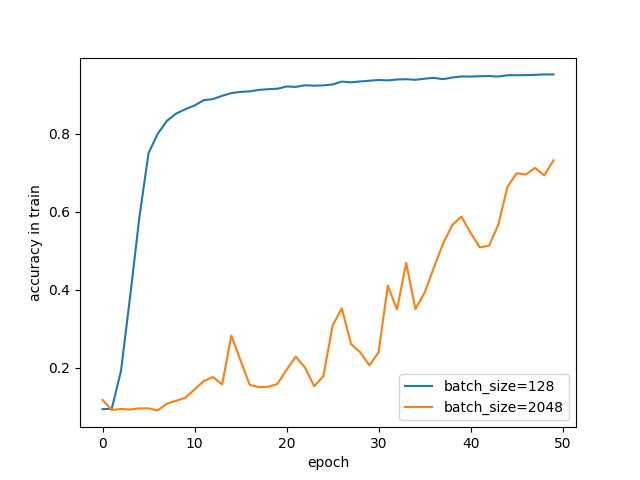
\includegraphics [scale=0.5]{local_batch_size_accuracy.png}
    \caption {batch size in locally connected layer}
\end{figure}
\newpage

(3) CNN: To test the parameter choice, 2\textit{batch size} of $[128, 4096]$ are
tested, the performance is given in Fig.9, we can see 
\textit{batch size=128} is more appropriate, and 
\textit{batch size=4096} will lead to slow learning and bad final performance.\\
\begin{figure}[h]
    \centering
    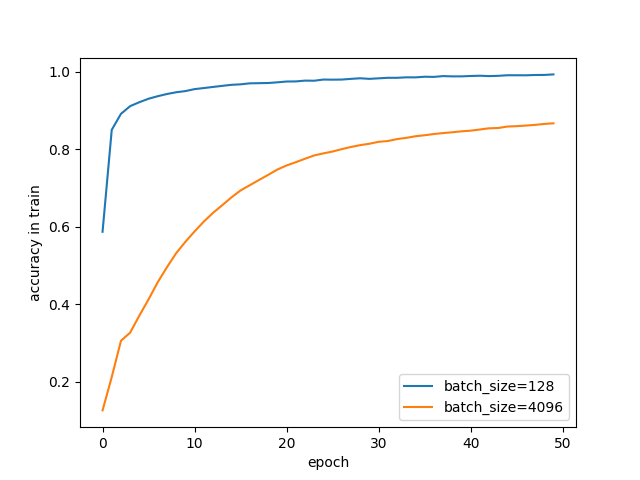
\includegraphics [scale=0.5]{cnn_batch_size_accuracy.png}
    \caption {batch size in CNN}
\end{figure}
\newpage

\subsection{Momentum}
Three values $[0.5, 0.9, 0.99]$ of momentum are tested on these 3 net
works.
\begin{figure}[h]
    \centering
    \begin{subfigure}[b]{0.32\linewidth}
    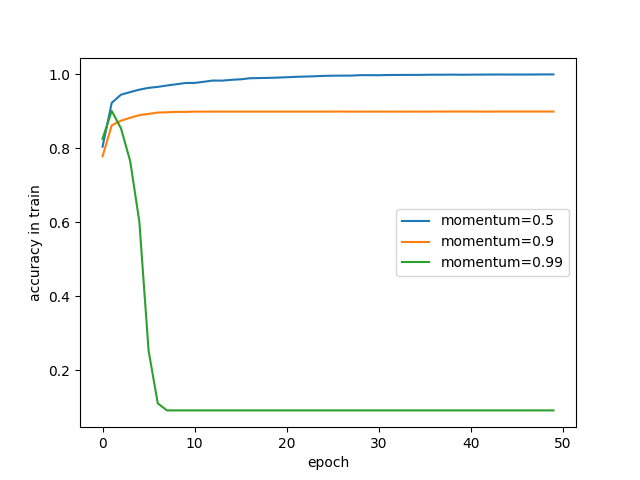
\includegraphics [width=\linewidth]{mlp_momentum_accuracy.png}
    \caption {MLP}
    \end{subfigure}
    \begin{subfigure}[b]{0.32\linewidth}
    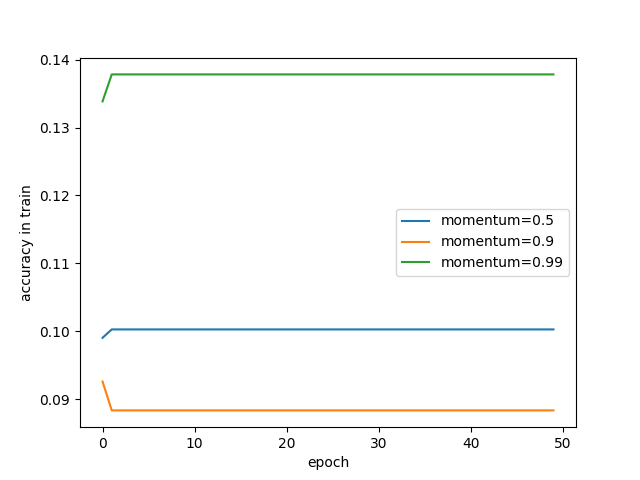
\includegraphics [width=\linewidth]{local_momentum_accuracy.png}
    \caption {Local}
    \end{subfigure}
    \begin{subfigure}[b]{0.32\linewidth}
    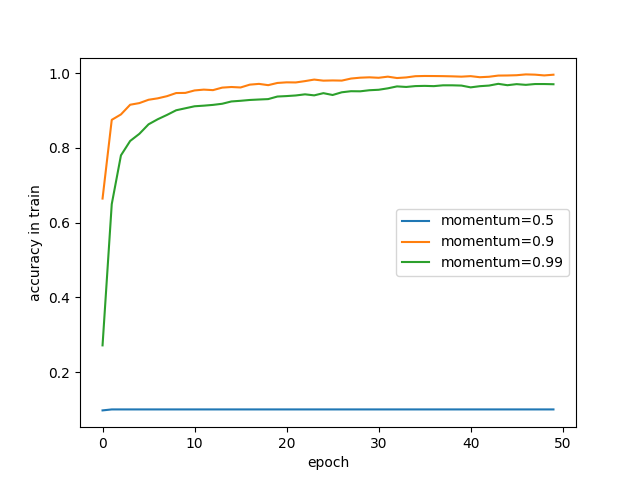
\includegraphics [width=\linewidth]{cnn_momentum_accuracy.png}
    \caption {CNN}
    \end{subfigure}
    \caption {momentum effects}
\end{figure}
The momentum effects varies on the 3 networks:\\
For MLP, \textit{momentum=0.9} will degrade the final performance, and it seems 
it arrives at plateau sooner then \textit{momentum=0.5}. \textit{momentum=0.99} 
leads to a failed learning.\\
For locally connected layer, all three momentum values leads to a failed learning.
Since the momentum actually acts as a accumulation of prior gradients, we can naively
understand it as equivalent to a increased batch size effect. The
learning immediately falls to local minimum, and bad performance is
observed.\\
For CNN, a very different behavior is observed. textit{momentum=0.9} has the best
 performance, \textit{momentum=0.5} performs slightly worse, and 
 \textit{momentum=0.99} leads to a failed learning.\\

\section{Techniques for improving generalization}
\subsection{ensemble networks}
To improve the generalization performance, 6 CNN networks are trained
independently. They have same architecture and differs in their
initialization of their weights. Once they are trained, they are ensembled to predict
the test set. As we can see in the table, the ensemble net has the
highest test accuracy then all the 6 networks. Ensemble increase the
final generalization capability.
\begin{table}[h]
    \caption{Test accuracy}
    \centering
    \begin{tabular}{c c c c c c c c}
        \hline\hline
        Networks & 1 & 2 & 3 & 4 & 5 & 6 & ensemble \\
        \hline
        Accuracy & 0.849 & 0.848 & 0.847 & 0.845 & 0.854 & 0.845 & \bm{0.856} \\
        \hline
    \end{tabular}
\end{table}

\subsection{Dropout}
During training, multiple realization of Dropout generates ensemble of
networks, and these networks share hidden units in training. In such a
way, it can generally improve the generation performance.
(1) Fully connected NN (MLP): To test the parameter choice, 2 \textit{dropouts} of 
$[0.2, 0.5]$ are tested, and in comparison, no dropout is also
included. The performance is given in Fig.11, we can see Dropout
degrade the trainning performance, but an appropriate chosen dropout
probalbility of 0.2 does not harm the test performance, while dropout
of 0.5 is too large and harms the trainning and generalization
significantly.
\begin{figure}[h]
    \centering
    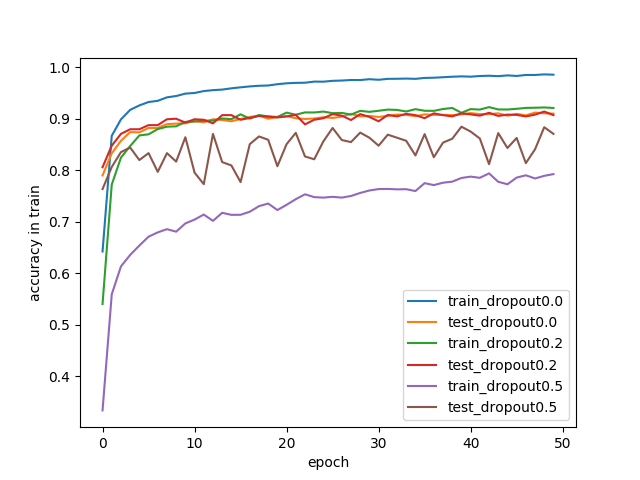
\includegraphics [scale=0.5]{mlp_dropout_accuracy.png}
    \caption {dropout effects in MLP}
\end{figure}
\newpage

(2) Locally connected NN: To test the parameter choice, 2 \textit{dropouts} of
$[0.2, 0.6]$ are tested, and in comparison, no dropout is also
included. The performance is given in Fig.12, we can see Dropout
degrade the trainning performance, but an appropriate chosen dropout
probalbility of 0.2 does not harm the test performance, while dropout
of 0.6 is too large and harms the trainning and generalization.
\begin{figure}[h]
    \centering
    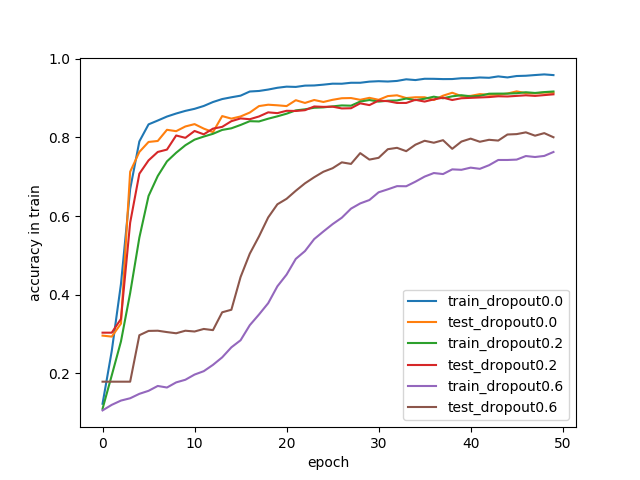
\includegraphics [scale=0.5]{local_dropout_accuracy.png}
    \caption {dropout effects in locally connected layer}
\end{figure}
\newpage

(3) CNN: To test the parameter choice, 2\textit{dropout} of
$[0.2, 0.6]$ are tested, and in comparison, no dropout is also
included. The performance is given in Fig.13, we can see Dropout
degrade the trainning performance, but an appropriate chosen dropout
probalbility of 0.2 does not harm the test performance, while dropout
of 0.6 is too large and harms the trainning and generalization, although
 it seems it still can catch up if we keep training.
\begin{figure}[h]
    \centering
    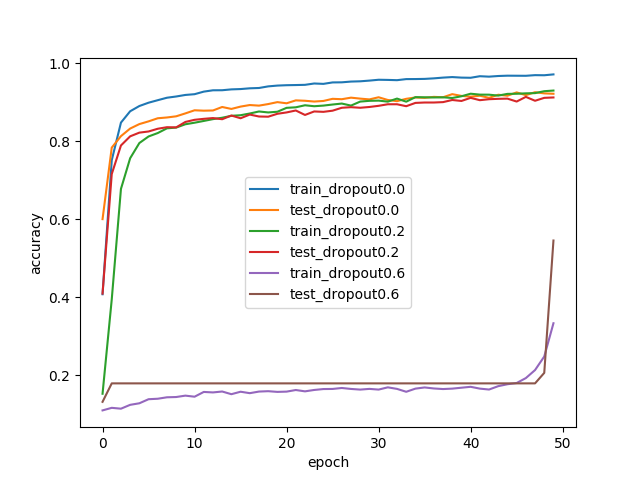
\includegraphics [scale=0.5]{cnn_dropout_accuracy.png}
    \caption {dropout effects in CNN}
\end{figure}
\newpage

\subsection{L1 regularization}
L1 regularization is known as introducing sparsity in the network, it
acts like feature selection and only keeps the significant weights.\\
(1) Fully connected NN (MLP): To test the parameter choice, 2 \textit{regularization}
of $[0.1, 0.2]$ are tested, and in comparison, no regularization is also
included. The performance is given in Fig.14, we can see L1
regularization degrade the trainning performance, but an appropriate chosen L1
regularization of coefficient 0.1 does not harm the test performance, while L1
coefficient of 0.2 is too large and harms the trainning and generalization
significantly. Eventually too many zeros are introduced in the network
and it failed to train at last for coefficient of 0.2.
\begin{figure}[h]
    \centering
    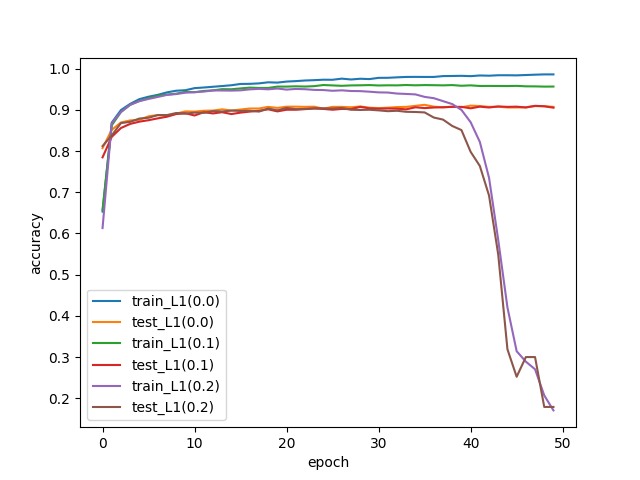
\includegraphics [scale=0.5]{mlp_regularization_accuracy.png}
    \caption {L1 regularization effects in MLP}
\end{figure}
\newpage

(2) Locally connected NN: To test the parameter choice, 2 \textit{regularization} of
$[0.0005, 0.002]$ are tested, and in comparison, no regularization is also
included. The performance is given in Fig.15, we can see L1
regularization degrade the test performance, even if we have a
coefficient as small as 0.0005. Coefficient of 0.002 further decrease
the final test accuracy. It seems L1 regularization is very dangerous
for locally connected net work and can lead to disasters if we chose
coefficients carelessly.
\begin{figure}[h]
    \centering
    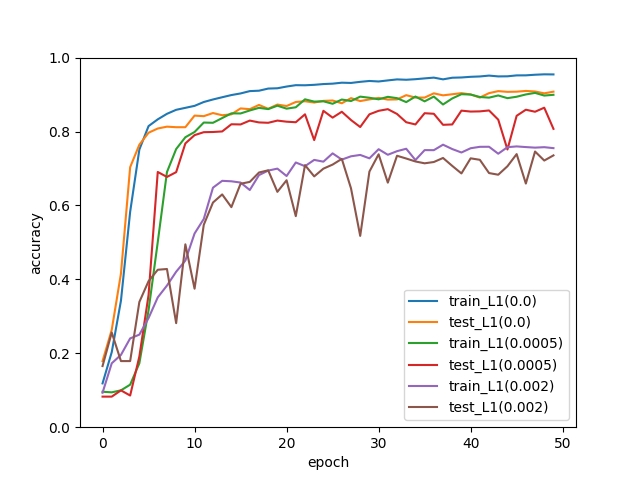
\includegraphics [scale=0.5]{local_regularization_accuracy.png}
    \caption {L1 regularization effects in locally connected layer}
\end{figure}
\newpage

(3) CNN: To test the parameter choice, 2\textit{regularization} of
$[0.01, 0.02]$ are tested, and in comparison, no regularization is also
included. The performance is given in Fig.16, we can see L1
regularization degrade the test performance. Coefficient of 0.02 further decrease
the final test accuracy and slower the learning. But it's relatively robust to L1
regularization compared with locally connected layer. 
\begin{figure}[h]
    \centering
    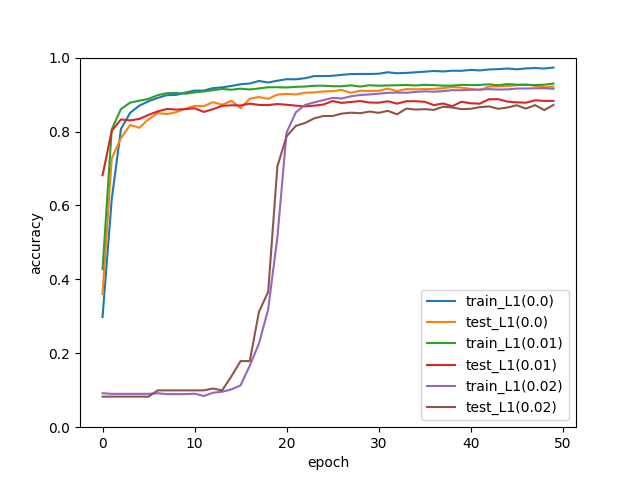
\includegraphics [scale=0.5]{cnn_regularization_accuracy.png}
    \caption {L1 regularization effects in CNN}
\end{figure}

\end{document}


